%%%%%%%%%%%%%%%%%%%%%%%%%%%%%%%%%%%%%%%%%%%%%%%%%%%%%%%%%%%%%%%%%%%%%%%%%%%%% 
%
% This is a LaTeX file for an A3 poster.
%
%%%%%%%%%%%%%%%%%%%%%%%%%%%%%%%%%%%%%%%%%%%%%%%%%%%%%%%%%%%%%%%%%%%%%%%%%%%%% 

%%%%%%%%%%%%%%%%%%%%%%%%%%%%%%%%%%%%%%%%%%%%%%%%%%%%%%%%%%%%%%%%%%%%%%%%%%%%% 
%%%%%%%%%%%%%%%%%%%%%%%%%%%%%%%%%%%%%%%%%%%%%%%%%%%%%%%%%%%%%%%%%%%%%%%%%%%%%
%
% Asymptotic behavior of solutions to the generalized Becker-Döring
% equations for general initial data.
%
% Poster for the HYKE-3 meeting in Rome, 13-15 April 2005.
% 
%%%%%%%%%%%%%%%%%%%%%%%%%%%%%%%%%%%%%%%%%%%%%%%%%%%%%%%%%%%%%%%%%%%%%%%%%%%%%
%%%%%%%%%%%%%%%%%%%%%%%%%%%%%%%%%%%%%%%%%%%%%%%%%%%%%%%%%%%%%%%%%%%%%%%%%%%%%

\documentclass{article}
% To modify the size of the page:
\usepackage[dvips,a3paper,landscape,centering,margin=1.1cm]{geometry}
\usepackage{multicol}
\usepackage[utf8]{inputenc}
\usepackage{color}

\usepackage{amsmath, amsthm, amsfonts}
\usepackage{graphicx}           % Include figure files.
\newtheorem{theorem}{Theorem}
\newtheorem{assertion}[theorem]{Assertion}
\newtheorem{claim}[theorem]{Claim}
\newtheorem{conjecture}[theorem]{Conjecture}
\newtheorem{corollary}[theorem]{Corollary}
\newtheorem{definition}[theorem]{Definition}
\newtheorem{proposition}[theorem]{Proposition}
\newtheorem{example}[theorem]{Example}
\newtheorem{figger}[theorem]{Figure}
\newtheorem{lemma}[theorem]{Lemma}
\newtheorem{prop}[theorem]{Proposition}

\usepackage[ruled,vlined]{algorithm2e}
\usepackage{tabularx}
\usepackage{longtable}
%\usepackage{booktabs}
\usepackage{multirow}
\usepackage{float}
\usepackage{tikz}
\usetikzlibrary{arrows}
\usetikzlibrary{shapes}
\usepackage{forest}
\newenvironment{treerow}{}{}
%\usepackage{smartdiagram}  
\usepackage{smartdiagram}
\usetikzlibrary{arrows.meta, positioning}
\usepackage{caption}
% Colors
% -------
\definecolor{azulillo}{rgb}{0.8,0.85,1}
\definecolor{marronrp3}{rgb}{.9,.9,.7}
\definecolor{salmon}{rgb}{1,.9,.8}
\definecolor{rojo}{rgb}{.6,.1,0}

\pagestyle{empty}

\def\to{\rightarrow}

% Hyphenation
\hyphenation{coa-gu-la-tion frag-men-ta-tion}

% ===========================================================================

\title{}
\author{}
\date{}

\begin{document}
\pagecolor{salmon}
%\maketitle
\begin{center}
  \begin{minipage}{.19\linewidth}
    
\includegraphics[width=.5\linewidth]{iitb1.png}
  \end{minipage}
  %&
  \begin{minipage}{.6\linewidth}
    \begin{center}
      \Huge \textbf{Similarity-based Lexicographic Method for Hierarchical Multiobjective Linear Programs}
    \end{center}
    \begin{center}
      \huge \underline{{\it Devanand R, Ashutosh Mahajan and N. Hemachandra}}
    \end{center}
    
  \end{minipage}
  %&
  \hspace{.03\linewidth}
  \begin{minipage}{0.16\linewidth}
    \begin{flushright}
      \large \underline{\textbf{Department}}\\
      Industrial Engineering and Operations Research, \\
      IIT Bombay, India\\
      \vspace{.1cm} \small \emph{\textbf{Acknowledgment:} I thank Tushar Shekhar, my external advisor, and manager at Blue Yonder, for his support and suggestions.}
    \end{flushright}
  \end{minipage}
\end{center}
\vspace{.1cm}

% ---------------------------------------------------------------------------

\setlength{\columnsep}{1cm}
\begin{multicols}{3}
\noindent
\fcolorbox{rojo}{marronrp3}{
  \begin{minipage}[t]{.96\linewidth}
    \vspace{.05cm}
    \begin{center}
      \vspace{.1cm}
      \section*{\Large \underline{At High Level}}

      \large We define the {\bf concept of similarity} between intermediate linear programs (LPs) appearing while solving the hierarchical multiobjective linear program ({\bf h-MOLP}) for the decision of whether we should solve the current LP from {\bf scratch} or use the {\bf available feasible solution} obtained from the {\bf previous} LP solve.
    \end{center}
  \end{minipage}
}
\section*{h-MOLP with bounded variables}
\vspace{-.4cm}
  \begin{minipage}[t]{.96\linewidth}
      \Large
      \begin{center}
 	\begin{align}
%\min f(x) = ({c^1}^{\tt{T}}x, & 
	\tt{lexmin~}{c^1}^{\tt{T}}&x,  ~{c^2}^{\tt{T}}x, \cdots, ~{c^t}^{\tt{T}}x  \nonumber  \\
	\mbox{subject to ~} & Ax = b, \nonumber \\ %\tag{h-MOLP} \\ 
	l \leq & x \leq  u. \nonumber 
 	\end{align}
	\end{center}
  \end{minipage}
{\large
  {\bf lexmin}: ${c^1}^{\tt{T}}x$ is more important than ${c^2}^{\tt{T}}x$ which is, more important than ${c^3}^{\tt{T}}x$, and so on and, ${c^t}^{\tt{T}}x$ is of least importance.
}
%{\textcolor{rojo} {\large {\bf Assumption} h-MOLP is nontrivial - we obtain alternative optimal solutions while solving the
%underlying LPs hierarchically, and objectives to those LPs conflict with each other.}}

\vspace{.1cm}
\noindent
 \underline{\Large {\bf Lexicographic Methods}}
\begin{enumerate}
\large
 \item $\mbox{~LP}^{k}$ - Constraint-addition rule 
 \item $\mbox{~modLP}^{k}$ - Variable fixing rule 
\end{enumerate}
\vspace{-.1cm}
\noindent
\begin{center}
\large 
\fcolorbox{rojo}{marronrp3}{
% 
  %\begin{minipage}[t]{.96\linewidth}
%\begin{center}
\begin{minipage}{0ex}
\begin{alignat}{2}
\mbox{~LP}^{k}:=\min & ~{c^{k}}x   \nonumber \\
\mbox{s.t. ~} Ax  =& b,\nonumber \\
{c^i}x  =& {y^i}, ~i = 1,\ldots, k-1, \nonumber \\
 l \leq  x &\leq  u. \nonumber
%\tag{$\tt{LP^k}$}, 
\end{alignat}
\end{minipage}
\hskip -7ex
\begin{minipage}{40ex}
\begin{alignat}{2}
\mbox{~modLP}^{k}:=\min  &~{c^k}x   \nonumber \\
\mbox{s.t. ~} &Ax  = b, \nonumber\\
 x_{j}  =& f_{j},~ j \in J^k \subseteq \{1,\ldots,n \}, \nonumber \\
l\leq  x &\leq  u. \nonumber
\end{alignat}
\end{minipage}
}
\end{center} 
{\Large \textbf{\underline{Remarks}}}
\begin{enumerate}
\large
\item Both provide Pareto-optimal solution
\item Most literature describes $\mbox{~LP}^{k}$ rule in the discussion of the method
\item Most solvers prefer implementing the $\mbox{~modLP}^{k}$
\item Assumption: h-MOLP is nontrivial - alternative optimal solutions while solving the underlying LPs, and we have conflicting objectives
\end{enumerate}
\section*{{\Large \underline{Motivation}}}
%\begin{itemize}
%\item Pareto optimal result: The constraint-addition and variable-fixing
%\item Ill-posed behavior: constraint-addition rule (high), variable-fixing rule (low) 
%\item basis matrix unchanged in two consecutive LPs in the variable-fixing rule
\vspace{-.2cm}
\noindent
\begin{itemize}
\large 
\item To obtain {\bf one solution} point both need the solution of {\bf many LPs} 
\item To {\bf speed it up}, many solvers provide a feature of {\bf Reoptimization} 
\item However, a rule is required to {\bf selectively decide} when to use Reoptimization 
\end{itemize}
%\item  However, sometimes it is better to avoid this and start afresh.
%\end{itemize}
%\vspace{.1cm}
\noindent
\begin{minipage}{40ex}
%%%%%%%%%%%%%%%%%%%%%%%
\begin{center}
   % \large{
\begin{figure}[H]
\centering 
 \resizebox{1.0\textwidth}{!}{%
 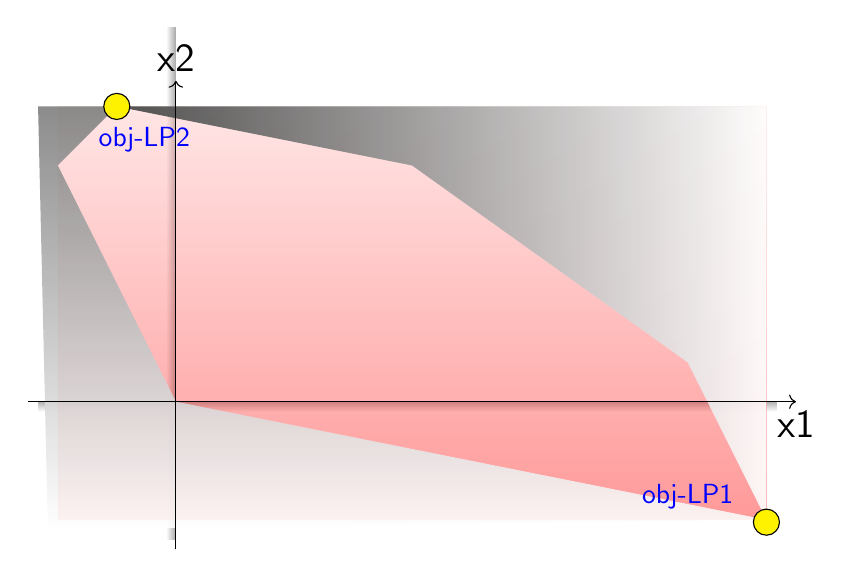
\begin{tikzpicture}[
    every path/.style = {},
    every node/.append style = {font=\sffamily}
  ]
 \begin{scope}[shift={(0,0)}]  %\draw[right color=gray, left color=white, opacity=0.7]
     % (-0.5,-0.5) rectangle (0,6.5);
    \shade[right color=gray, left color=white, opacity=0.7]
      (-0.125,-1.75) rectangle (0,4.75);
    
    \shade[top color=gray, bottom color=white, opacity=0.6]
      (-1.75,-0.125) rectangle (7.625,0);
       
   \shade[top color=pink, bottom color=red, opacity=0.4]
      (-1.5,-1.5) rectangle (7.5,3.75);
   
    \shade[left color=darkgray, top color=gray, opacity=0.9]
      (7.5,-1.5)--(0,0)--(-1.5,3)--(-0.75,3.75)--(-1.75,3.75)--(-1.625,-1.625) -- cycle;
    
    \shade[left color=darkgray, right color=white, opacity=0.9]
     (-0.75,3.75) -- (7.5,3.75) -- (7.5,-1.5) -- (6.5,0.5) -- (3,3) -- cycle;
        
%    \draw[line width=0.5mm,yellow] (7.5,-1.5)--(6.5,0.5);
%    \draw[line width=0.7mm,yellow] (6.5,0.5)--(3,3); 
%    \draw[line width=0.7mm,yellow] (3,3)--(-0.75,3.75);
%    \draw[line width=0.7mm,yellow] (-0.75,3.75)--(-1.5,3);
     %\node[yshift=0.0cm, blue] at (1.6,5.3){Constraint 1};
      %\draw[line width=0.5mm,blue] (0,0.75)--(1.375,2.375);
     
      \node[yshift=0.0cm, blue] at (6.5,-1.2){obj-LP1};  
     \node[draw,circle, fill=yellow,minimum size=.2mm] at (7.5,-1.53) {};
     
    \node[yshift=0.0cm, blue] at (-0.4,3.325){obj-LP2};  
    \node[draw,circle, fill=yellow,minimum size=.2mm] at (-0.75,3.75) {};      
   \draw[->] (-1.875,0) -- (7.875,0) node[below] {{\Large x1}};
    \draw[->] (0,-1.875) -- (0,4.075) node[above] {{\Large x2}};
%    \foreach \i in {-7,-5,...,15} {
%      \draw[help lines] (-6.5,\i) -- (31,\i);
%    }
%    \foreach \i in {-7,-5,...,31} {
%      \draw[help lines] (\i,15) -- (\i,-6.5);
%    }
%    \foreach \i in {-7,-5,...,16} {
%      \node[label={left:\i}] at (0,\i){};
%    }
%    \foreach \i in {-7,-5,...,30} {
%      \node[below] at (\i,-0.2) {\pgfmathparse{int(\i)}\pgfmathresult};
%    }

   % \node[very thick, draw=black, fill=white, rectangle, rounded corners,
    %  text width=7em, align=center] at (26.5,7.5)
    %  {Feasible regions are the black lines in the pink colored area};
   
   % \node[very thick, draw=black, fill=white, rectangle, rounded corners,
     % text width=6em, align=center] at (5,5)
     % {Feasible solutions of the integer program are the black dots};
  \end{scope}
\end{tikzpicture}
}
\caption*{Prefer Solving from Scratch}
%\label{ch1:pareto front}
\end{figure}
\end{center}
\end{minipage}
%~~and
\hskip 1ex
\begin{minipage}{40ex}

%%%%%%%%%%%%%%%%%%%%%%%
\begin{center}
   % \large{
\begin{figure}[H]
\centering 
 \resizebox{1.0\textwidth}{!}{%
 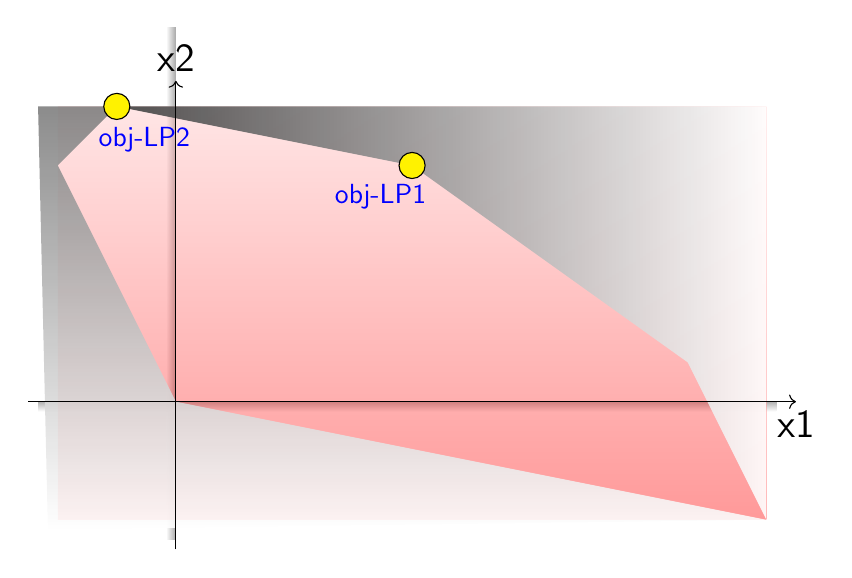
\begin{tikzpicture}[
    every path/.style = {},
    every node/.append style = {font=\sffamily}
  ]
 \begin{scope}[shift={(0,0)}]  %\draw[right color=gray, left color=white, opacity=0.7]
     % (-0.5,-0.5) rectangle (0,6.5);
    \shade[right color=gray, left color=white, opacity=0.7]
      (-0.125,-1.75) rectangle (0,4.75);
    
    \shade[top color=gray, bottom color=white, opacity=0.6]
      (-1.75,-0.125) rectangle (7.625,0);
       
   \shade[top color=pink, bottom color=red, opacity=0.4]
      (-1.5,-1.5) rectangle (7.5,3.75);
   
    \shade[left color=darkgray, top color=gray, opacity=0.9]
      (7.5,-1.5)--(0,0)--(-1.5,3)--(-0.75,3.75)--(-1.75,3.75)--(-1.625,-1.625) -- cycle;
    
    \shade[left color=darkgray, right color=white, opacity=0.9]
     (-0.75,3.75) -- (7.5,3.75) -- (7.5,-1.5) -- (6.5,0.5) -- (3,3) -- cycle;
        
%    \draw[line width=0.5mm,yellow] (7.5,-1.5)--(6.5,0.5);
%    \draw[line width=0.7mm,yellow] (6.5,0.5)--(3,3); 
%    \draw[line width=0.7mm,yellow] (3,3)--(-0.75,3.75);
%    \draw[line width=0.7mm,yellow] (-0.75,3.75)--(-1.5,3);
     %\node[yshift=0.0cm, blue] at (1.6,5.3){Constraint 1};
     %\node[yshift=0.0cm, blue] at (6.5,-1.2){obj-LP2};  
     %\node[draw,circle, fill=yellow,minimum size=.2mm] at (7.5,-1.53) {};
     \node[yshift=0.0cm, blue] at (-0.4,3.325){obj-LP2};    
     \node[draw,circle, fill=yellow,minimum size=.2mm] at (-0.75,3.75) {};
 
    \node[yshift=0.0cm, blue] at (2.6,2.6){obj-LP1};  
    \node[draw,circle, fill=yellow,minimum size=.2mm] at (3,3) {};  
      
   \draw[->] (-1.875,0) -- (7.875,0) node[below] {{\Large x1}};
    \draw[->] (0,-1.875) -- (0,4.075) node[above] {{\Large x2}};
%    \foreach \i in {-7,-5,...,15} {
%      \draw[help lines] (-6.5,\i) -- (31,\i);
%    }
%    \foreach \i in {-7,-5,...,31} {
%      \draw[help lines] (\i,15) -- (\i,-6.5);
%    }
%    \foreach \i in {-7,-5,...,16} {
%      \node[label={left:\i}] at (0,\i){};
%    }
%    \foreach \i in {-7,-5,...,30} {
%      \node[below] at (\i,-0.2) {\pgfmathparse{int(\i)}\pgfmathresult};
%    }

   % \node[very thick, draw=black, fill=white, rectangle, rounded corners,
    %  text width=7em, align=center] at (26.5,7.5)
    %  {Feasible regions are the black lines in the pink colored area};
   
   % \node[very thick, draw=black, fill=white, rectangle, rounded corners,
     % text width=6em, align=center] at (5,5)
     % {Feasible solutions of the integer program are the black dots};
  \end{scope}
\end{tikzpicture}
}
\caption*{Prefer Reoptimization}
%\label{ch1:pareto front}
\end{figure}
\end{center}
\end{minipage}
% }
%\end{center}
%%%%%%%%%%%%%%%%%%%%%%%

%\begin{center}
%  \noindent
% \fcolorbox{rojo}{marronrp3}{
%\begin{minipage}{30ex}
%\begin{alignat*}{1}
%\mathbf{LP_{1}}:= ~\min_{x\in \mathbb{R}^{2}}{~x_{2}} &  \nonumber \\
%\mbox{subject to~~~~}\\ 3\leq x_{1}+x_{2} & \leq 9 \nonumber \\ 
%-3 \leq x_{1}-x_{2} & \leq 3 \nonumber \\
%x_{1} + 2x_{2} & \leq 13 \nonumber \\
%x_{1} - 2x_{2} & \geq -7 \nonumber 
%%\\\tag{LP1} 
%%\label{LP1} 
%\end{alignat*}
%\end{minipage}
%~~and
%\hskip 1ex
%\begin{minipage}{30ex}
%
% \begin{alignat*}{1}
%\mathbf{LP_{2}}:= ~\min_{x\in \mathbb{R}^{2}}{~-x_{2}} &  \nonumber \\
%\mbox{subject to~}\\ 3\leq x_{1}+x_{2} & \leq 9 \nonumber \\ 
%-3 \leq x_{1}-x_{2} & \leq 3 \nonumber \\
%x_{1} + 2x_{2} & \leq 13 \nonumber \\
%x_{1} - 2x_{2} & \geq -7 %\\\tag{LP2} 
%\end{alignat*}
%\end{minipage}
% }
%\end{center}
%%$\mathbf{LP_{1}}$ and $\mathbf{LP_{2}}$ have optimal solutions at $p^{\ast}=(3,0)$  and $q^{\ast}=(3,5)$ respectively. Moreover, to 
%To solve the problem $\mathbf{LP_{2}}$ by simplex method, it is not computationally beneficial to prefer the starting basic feasible solution as $p^{\ast}$, than to start with any other basic feasible solution of $\mathbf{LP_{2}}$. We see this case for both the primal and dual simplex methods.
%\vspace{.2cm}
\noindent
\textbf{\Large \underline{Notion of Similarity}}
\vspace{.1cm}

\noindent
 \fcolorbox{rojo}{marronrp3}{
\begin{minipage}[t]{.96\linewidth}
{\large $LP^1$ is {\bf similar} to $LP^2$, if the solution of $LP^1$ helps solve $LP^2$ faster than just solving it from scratch.} 
\end{minipage}
}
\begin{center}  
\begin{definition}
     Let $LP^1 := \min \{  {c^1}x ~|~ Ax = b, ~l^1 \leq x \leq u^1 %,~x^{11} = \tilde{x}^{11}, %~x^{11} \subseteq x
     \}$ and $LP^2 := \min\{  {c^2}x  ~|~  Ax = b,~ l^2 \leq x \leq u^2 %, ~x^{12} = \tilde{x}^{12}, %~x^{12} \subseteq x, ~ x^{12} \neq \emptyset ~\&~ x^{11} \subset x^{12} 
     \}$ are two LPs.  
     We assume that the feasible sets of both $LP^1$ and $LP^2$ are non-empty.
     With respect to $p$ and $B$, the optimal solution and the optimal basis of $LP^1$, we say $LP^1$ and $LP^2$ are ``similar'' if  
             $$\Big[ 1 -  \big( \frac{\sum_{j=1}^n I_{p_{j}}|c^2_j - c^1_j|}{\sum_{j=1}^n |c^2_j - c^1_j|}\big) \Big] \geq \kappa,$$ where $0 \leq \kappa \leq 1$ is the given parameter. $I_{p_{j}}$ the indicator function is equal to 1 if $e_j \neq 0 \text{~and~} \overline{c^1_j} = 0$, else is set to 0. Here, reduced cost of $LP^1$ is $\overline{c^1} := c^1 - c^1_B B^{-1}A$ and $e: =  c^2 - c^2_B B^{-1}A$ is assumed as the estimated reduced cost of $LP^2$.
\end{definition}
\end{center}

\begin{center}
\large
\fcolorbox{rojo}{marronrp3}{
  \begin{minipage}[t]{.96\linewidth}
%\begin{proposition}
\textbf{\Large \underline{Result}}\\
%Suppose $LP^1 = \min \{  {c^1}x ~|~ Ax = b, ~l^1 \leq x \leq u^1 %,~x^{11} = \tilde{x}^{11}, %~x^{11} \subseteq x
%     \}$ is a linear program.  
%Consider $p, B$ and $\overline{c^1}$ are the optimal solution, solution basis and reduced costs information respectively %at optimality 
%of $LP^1 %~min~ {c^1}^Tx;  ~s.t.~ Ax = b, ~l \leq x \leq u
%$. 
Consider $p, B$ and $\overline{c^1}$ are at optimality of $LP^1$.
Consider %an LP with 
a perturbed cost vector $c^2 = c^1 + \delta$ %and %perturbed reduced cost $\overline{c^2}$, 
where $\delta \neq 0$ is given. 
Let $e = c^2 - c^2_B B^{-1} A$.
For any component $p_i, i \in \{1,\dotsc,n\}$, if $\overline{c_i^1} \cdot e_i \leq 0$ and, %\{i~|
$\overline{c_i^1}$ and $e_i$ both can not together be zero, 
%\} = \emptyset
%$, 
the basis $B$ of $LP^1$ is not the optimal basis of $LP^1$ with perturbed cost vector $c^2$. 
%\end{proposition}
\end{minipage}
}
\end{center}

% ---------------------------------------------------------------------------
\noindent
\textbf{\Large \underline{SimLex: Similarity-based Decision to Reoptimize}}
\vspace{-.1cm}
%\section*{Similarity-based decision to reoptimize}
\begin{center}
\begin{minipage}[t]{.96\linewidth}
   % \large{
\begin{figure}[H]
\centering 
 \resizebox{0.6\textwidth}{!}{%
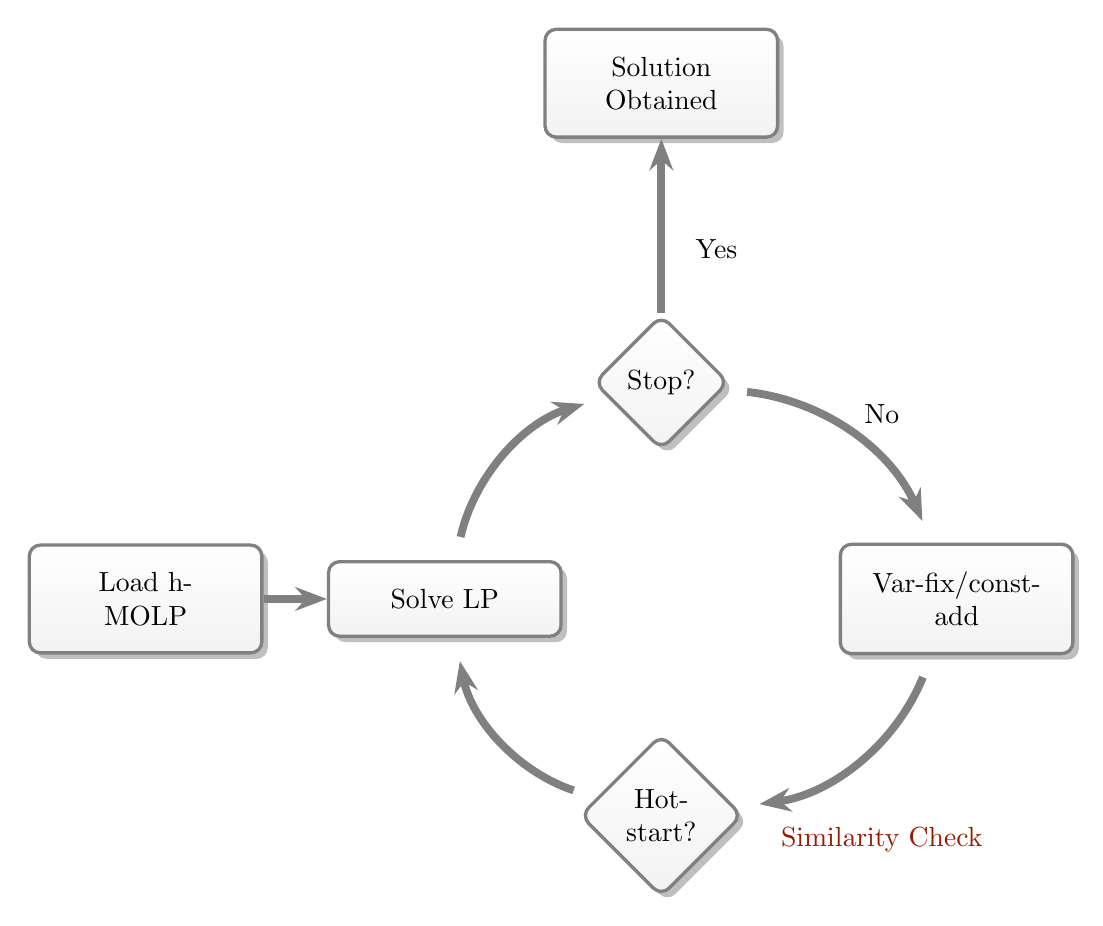
\begin{tikzpicture}[auto]  
\tikzset{
    mynode1/.style={diamond,rounded corners, draw=gray, top color=white,
                   bottom color=white!90!gray,very thick, inner sep=1mm,
                   minimum size=1mm, text centered, minimum width=1.00cm, 
                   drop shadow, text width=1.00cm},
    mynode2/.style={rectangle,rounded corners, draw=gray, top color=white,
                   bottom color=white!90!gray,very thick, inner sep=1em,
                   minimum size=1em, text centered, minimum width=2.3cm, 
                   drop shadow, text width=2.25cm},
    myleft/.style={-{Stealth[length=4mm]}, color=gray, line width=0.1cm, 
                   draw, shorten <=0.3cm,shorten >=0.3cm, bend left},
   mystrt/.style={-{Stealth[length=4mm]}, color=gray, line width=0.1cm, 
                   draw},
}

\node[mynode2] at ([yshift=2.75cm] 0:-6.55cm)(start) {Load h-MOLP};
\node[mynode2] at ([yshift=2.75cm] 90:6.55cm)(stop) {Solution Obtained};
\node[mynode1] (hotSt) {Hot-start?};
\node[mynode2] at ([yshift=2.75cm] 0:3.75cm) (varf) {Var-fix/const-add};
\node[mynode1] at ([yshift=2.75cm] 90:2.75cm) (stopCrit) {Stop?};
\node[mynode2] at ([yshift=2.75cm] 180:2.75cm) (solveLP) {Solve LP};

\node[yshift=0.0cm, black] at (0.7,7.2){Yes}; 
\node[yshift=0.0cm, black] at (2.8,5.1){No}; 
\node[yshift=0.0cm, rojo] at (2.8,-0.3){Similarity Check}; 
\path[mystrt] (start) to (solveLP);
\path[myleft] (hotSt) to (solveLP);
\path[myleft] (solveLP) to (stopCrit);
\path[mystrt] (stopCrit) to (stop);
\path[myleft] (stopCrit) to (varf);
\path[myleft] (varf) to (hotSt);
\end{tikzpicture} 
}
%\caption{Iterative LP solves in LM with hot-start}
%\label{ch1:reoptinhMOLP}
\end{figure}
  \end{minipage}
\end{center}
\noindent
%\noindent
%\begin{center}
%\begin{minipage}[t]{.96\linewidth}
%\begin{algorithm}[H]
%%\SetAlgoLined
%\KwIn{Feasible set $\tt{F} := \{ x~|~ Ax = b, l \leq x \leq u \}$; List of $K$ %objective coefficient 
%vectors
%%, each associated with objective function, indexed with highest to lowest priority 
%$%C := 
%[{c^1}, \dotsc,{c^K}]$. }
%\KwOut{List of $K$ solutions for each objectives, %of $C$
% $\tt{S} :=[{y^{1}}, \dotsc, {y^{K}}]$: 
%%${c^i}^{\tt{T}}x, k = 1,\dotsc,K $
%}
%%
%Solve $\tt{{LP}^{1}}:=  \min \{ {c^1}x | x \in  \tt{F} \}$ and store the its solution ${y^{1}}$ to $\tt{S}$. \\
%Update $\tt{F}$ using the solution obtained from $\tt{LP^{1}}$.\\
%\For{$k = 2,\dotsc,k$}{
%  \eIf{$\tt{{LP}^{k}}:= \min \{{c^k}x | x \in  \tt{F} \}$ and $\tt{{LP}^{k-1}}$ are similar (w.r.t $y^{k-1}$)}{
%   Solve $\tt{{LP}^{k}}$ with starting solution information $y^{k-1}$ \;
%   }{
%   Solve $\tt{{LP}^{k}}$ from scratch. \;
%   }
%   Save the current solution $y^k$ in $\tt{S}$ \;
%  }
%Return $\tt{S}$ as the final solution to the given input problem.
% \caption{SimLex}
%\end{algorithm}
%%\colorbox{marronrp3}{ 
%  \end{minipage}
%%}
%\end{center}
\vspace{-0.6cm}
\begin{center}
\centering
  %\begin{minipage}[t]{.96\linewidth}
\begin{figure}[H]
\begin{center}
    \includegraphics[width=0.8\linewidth]{SC1I2h.png}
\end{center}
\caption*{{\large {\bf Performance comparison}: SimLex Vs Variable-fixing. Blue points at level 1 indicate solving with hotstart and at level 0 indicate solving from scratch}}
\end{figure} 
 %\end{minipage}
  \end{center}
\vspace{-.1cm}
\noindent
 \underline{\Large {\bf Result and Future Work}}
\begin{center}
\large
\begin{minipage}[t]{.96\linewidth}
\begin{enumerate}
%\item Validate the idea on \textbf{MOPLIB}, a problem library for multi-objective linear, multi-objective (mixed) integer and vector linear programs
\item Comparison is done over default CPLEX12.10 and other rules 
\item Apply this idea with  1) \textbf{MOPLIB}, a library of benchmark multi objectives programs, and, 2) model of the \textbf{master production schedules} (MPS)
\item Reported {\bf 25\%} (SGM-50) speedup from our rule over default CPLEX rule on obtaining MPS on {\bf 13} large scaled {\bf consumer and products goods} (CPG) industry dataset  
\item {\bf Ideal parameter selection} of $\kappa$ for similarity computation is not emphasized and is the main works that need to be done  
\end{enumerate}
\end{minipage}
\end{center}
%\begin{center}
%\begin{table}[H]
%\begin{center}
%\caption{No. of iterations to solve: Our idea with different $\kappa$ over default CPLEX 12.10 and other rules, Dataset: MOPLIB, a problem library for multi-objective linear, multi-objective (mixed) integer and vector linear programs}
%\scalebox{0.63}{
%\begin{tabular}{l|l|l|l|l|l|l|l|l|l|l|l|l|l}
%\hline
%\multicolumn{1}{c|}{} & \multicolumn{1}{|c|}{} & \multicolumn{1}{|c|}{} & \multicolumn{1}{|c|}{} &
%\multicolumn{10}{c}{simlex} \\
%\hline
%\multicolumn{1}{c|}{instance} & \multicolumn{1}{|c|}{def-cplex} & 
%\multicolumn{1}{|c|}{const-add} & \multicolumn{1}{|c|}{var-fix} & 0.1 & 0.2 & 0.3 & 0.4 & 0.5 & 0.6 & 0.7 & 0.8 & 0.9 & 1 \\
%\hline
%\begin{tabular}[c]{@{}l@{}}molp\_3\_100\_20\_ - \\ assignment\end{tabular}  & \textbf{14} & 34 & 14 & 14 & 14 & 14 & 14 & 14 & 14 & 14 & 14 & \textbf{13} & \textbf{13} \\
%%\begin{tabular}[c]{@{}l@{}}molp\_4\_729\_729\_ - \\ bensolvehedron \end{tabular}  & \textbf{40} & \textbf{46} & 143 & 143 & 143 & 143 & 143 & 143 & 143 & 143 & 143 & 143 & 143 \\
%\begin{tabular}[c]{@{}l@{}}molp\_4\_900\_60\_ - \\ assignment \end{tabular}  & 99 & 212 & 99 & 99 & 99 & 99 & 99 & 99 & 99 & 99 & \textbf{97} & \textbf{97} & \textbf{97} \\
%\begin{tabular}[c]{@{}l@{}}molp\_9\_100\_60\_- \\ mpp \end{tabular}  & \textbf{65} & 81 & 77 & 77 & 77 & 77 & 77 & 77 & 77 & 81 & 84 & 90 & 99 \\
%%\begin{tabular}[c]{@{}l@{}}molp\_10\_779\_10174\_- \\ entropy \end{tabular}  & 42763 & 9300 & \textbf{6527} & \textbf{6527} & \textbf{6527} & \textbf{6527} & \textbf{6527} & \textbf{6527} & \textbf{6527} & \textbf{6527} & 23731 & 21902 & 21902 \\
%\begin{tabular}[c]{@{}l@{}}molp\_10\_900\_60\_- \\ assignment \end{tabular}  & 99 & 441 & 99 & 99 & 99 & 99 & 99 & 99 & 99 & 99 & \textbf{97} & \textbf{97} & \textbf{97} \\
%%\begin{tabular}[c]{@{}l@{}}molp\_12\_21\_30\_- \\  dc  \end{tabular} & \textbf{8} & 18 & \textbf{8} & \textbf{8} & \textbf{8} & \textbf{8} & \textbf{8} & \textbf{8} & \textbf{8} & \textbf{8} & \textbf{8} & \textbf{8} & \textbf{8} \\
%%\begin{tabular}[c]{@{}l@{}}molp\_21\_31\_138\_- \\  entropy \end{tabular} & 52 & 128 & \textbf{35} & \textbf{35} & \textbf{35} & \textbf{35} & \textbf{35} & \textbf{35} & 86 & 86 & 158 & 158 & 158 \\
%\begin{tabular}[c]{@{}l@{}}molp\_22\_43\_213\_- \\  entropy \end{tabular} & 113 & 160 & \textbf{97} & \textbf{97} & \textbf{97} & \textbf{97} & \textbf{97} & \textbf{97} & 100 & 100 & 219 & 219 & 219 \\
%\begin{tabular}[c]{@{}l@{}}molp\_23\_28\_218\_- \\  entropy \end{tabular} & 2 & 2313 & 3 & 3 & 3 & 3 & 3 & 3 & 1 & 4 & \textbf{0} & \textbf{0} & \textbf{0} \\
%\begin{tabular}[c]{@{}l@{}}molp\_27\_28\_218\_- \\  entropy \end{tabular} & 1 & 151 & 1 & 1 & 1 & 1 & 1 & 1 & 1 & \textbf{0} & \textbf{0} & \textbf{0} & \textbf{0} \\
%\hline
%\text{\begin{tabular}[c]{@{}l@{}}\# times beats %equal to \\      or 
%others\end{tabular}} & 4 & 1 & 4 & 4 & 4 & 4 & 4 & 4 & 2 & 3 & 5 & \textbf{6} & \textbf{6} \\
%\hline
%\end{tabular}
%}
%\label{solve:Benchmark}
%\end{center}
%\end{table}
%\end{center}
% ---------------------------------------------------------------------------
%
%\small
%\begin{thebibliography}{}
%
%\bibitem{BCP86} J. M. Ball, J. Carr, O. Penrose, \emph{The
%    Becker-D\"oring cluster equations: basic properties and asymptotic
%    behaviour of solutions}, Comm. Math. Phys. 104, 657--692 (1986)
%
%\bibitem{BC88} J. M. Ball, J. Carr, \emph{Asymptotic behaviour of
%    solutions to the Becker-D\"oring equations for arbitrary initial
%    data}, Proc. Roy. Soc. Edinburgh Sect. A, 108, 109-116 (1988)
%  
%\bibitem{C04} J. A. Cañizo, \emph{Asymptotic behavior of solutions to
%    the generalized Becker-Döring equations for general initial data},
%  preprint.
%  
%\bibitem{CdC94} J. Carr, F. P. da Costa, \emph{Asymptotic behaviour of
%    solutions to the coagulation-fragmentation equations. II. Weak
%    fragmentation}, J. Stat. Phys. 77, 89--123 (1994)
%
%\bibitem{dC98} F. P. da Costa, \emph{Asymptotic behaviour of low
%    density solutions to the generalized Becker-D\"oring equations},
%  NoDEA Nonlinear Differential Equations Appl. 5, 23--37, (1998)
%  
%\bibitem{LM} Ph. Lauren\c{c}ot, S. Mischler, \emph{Notes on the
%    Becker-D\"oring equation}, personal communication.
%
%\bibitem{LM02e} Ph. Lauren{\c{c}}ot, S. Mischler, \emph{From the
%    {B}ecker-{D}\"oring to the {L}ifshitz-{S}lyozov-{W}agner
%    equations}, J. Statist. Phys. 106, 5-6, pages 957--991 (2002).
%
%\end{thebibliography}

\end{multicols}
	
\end{document}